\documentclass[11pt]{article}
\usepackage{listings}
\usepackage{amsfonts}
\usepackage{graphicx}
\newcommand{\numpy}{{\tt numpy}}    % tt font for numpy

\topmargin -.5in
\textheight 9in
\oddsidemargin -.25in
\evensidemargin -.25in
\textwidth 7in

\begin{document}

% ========== Edit your name here
\author{Francesco Penasa}
\title{Homework-7}
\maketitle

\medskip

% ========== Begin answering questions here
\begin{enumerate}

\item
\textbf{Solution for WebGoat8/RequestForgeries/Cross-SiteRequestForgeries/7.}

In order to resolve exercise seven of the Cross-Site Request Forgeries in WebGoat8 we followed the instruction given in the exercise's page. One of the instruction contains the link \textit{pentestmonkey.net/blog/csrf-mxl-post-request} where an approach to a similar problem is addressed. The solution in such page consist to use \textit{enctype="text/plain"} to avoid the encoding of the html's body. 
We emulated such solution adding the \textit{enctype="text/plain"} attribute in our form, which is similar to the forms used in the previous exercises (exercises 3 and 4). 
The form modified in this way is the following.
\begin{lstlisting}[language=html]
<form name="attack" enctype="text/plain" method="POST"
action="http://localhost:8081/WebGoat/csrf/feedback/message">
	<input type="hidden" name='{
		"name": "WebGoat", 
		"email": "webgoat@webgoat.org", 
		"message": "WebGoat is the best!!"}'>
	<input type="submit" name="submit" value="Submit">
</form>
\end{lstlisting}
We open an \textit{.html} file that contains such form in the same browser that we have used to access the WebGoat exercise. 
Subsequently, we click on the submit button and the web browser will respond us with a JSON message containing the flag required in the exercise page.\\
The flag values in this case is: \textbf{1dec9d5b-3dee-4200-b0f9-adb1ee88edf1}\\
\\

In the following page a few screenshot of the html code and the result in WebGoat8 are displayed.


\begin{figure}
\centering
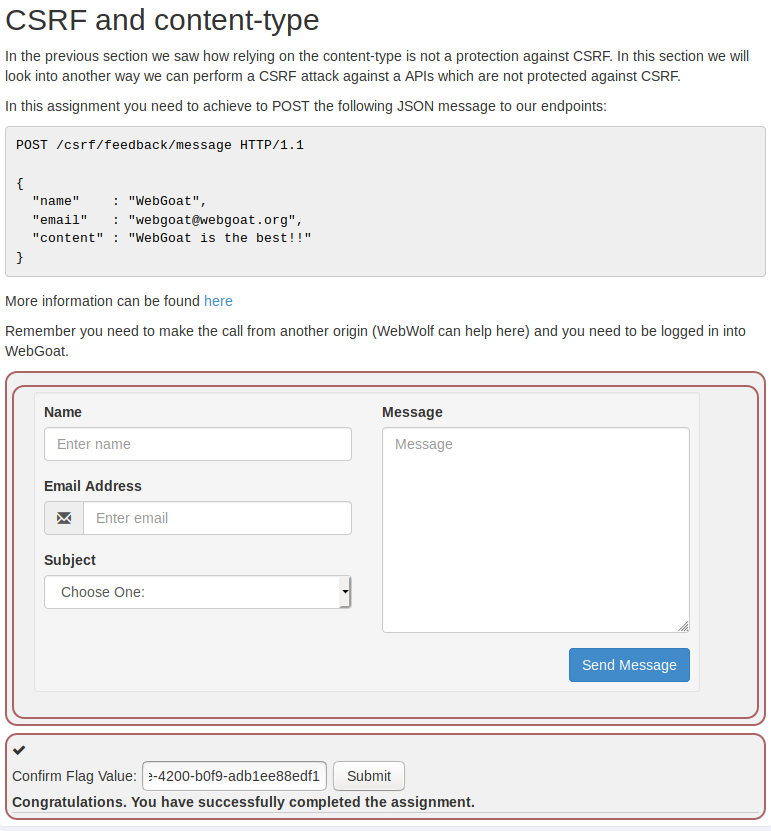
\includegraphics[scale=0.45]{result.png}
\end{figure}

\begin{figure}
\centering
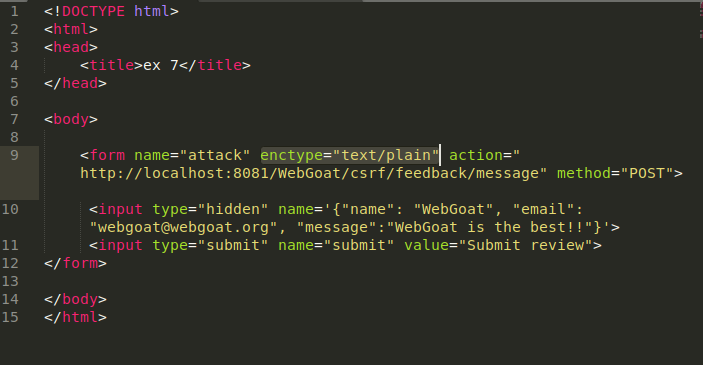
\includegraphics[scale=0.55]{html.png}
\end{figure}
\end{enumerate}
\end{document}
\grid
\grid